%%
%% licence       kaneton licence
%%
%% project       kaneton
%%
%% file          /home/buckman/kaneton/view/books/arch-ia32-virtual/bootloader.tex
%%
%% created       matthieu bucchianeri   [sat sep  2 11:40:18 2006]
%% updated       matthieu bucchianeri   [sat nov  4 16:43:05 2006]
%%

%
% bootloader
%

\chapter{Bootloader}

This chapter describes the boot phase of kaneton on IA-32 systems. The
early bootstrap is done using the GRand Unified Bootloader
(GRUB). This choice offers very flexible possibilities when installing
kaneton on a classical PC: GRUB supports booting on many filesystems,
even network. GRUB is very customizable and works with any kind of
hardware.

\newpage

%
% overview
%

\section{Overview}

Remember that the goal of the bootloader is to prepare the execution
environment in order to launch the kernel properly. Due to
compatibility reasons, Intel choosed to leave the boot mecanism as it
was in early computers in the 80's. This means that once the BIOS
jumps to the boot code, the microprocessor is still running in
\textbf{real-mode}, supporting poor addressing through a 20-bit
address bus.

Preparing a good environment for the kernel begins with switching to
\textbf{protected-mode} in order to address all the available memory
through the whole 32-bit address bus. Modern bootloaders like GRUB do
this job, so our task is just to prepare the \textbf{segmentation
environment}.

After, the bootloader needs to \textbf{reserve} a few memory areas for
the future kernel structures: from the \textit{init} structure to the
kernel execution stack. For better performances, the kernel and the
modules are compiled and linked with absolute addressing. This means
that we must \textbf{relocate} them to the address they were designed
to run from.

Then, as our implementation of kaneton is using virtual memory, we
must prepare a basic mapping before switching to \textbf{paging-mode}.

Once the processor is ready and the \textit{init} structure filled, we
can jump to the kernel.

%
% kernel and modules relocation
%

\section{Kernel and modules relocation}

The kernel code is compiled to be ran from a precise address. As GRUB
is loading the kernel and the modules at random addresses, we must
ensure that the kernel is copied to its \textbf{base address} and the
modules are grouped and dumped to an address above the 16 first
megabytes. The reason for copying everything above this limit and
working exclusively with addresses above 16 Mb is to keep the
beginning of the memory free, since some hardware using memory
accesses such as DMA can only address with 24-bits.

In order to determine the kernel base address, we need to read the
binary's ELF header. With this value, we are now able to copy the
kernel to a good location and to setup a simple page allocator. The
need of such allocator is to create structures like the \textit{init}
variable. This allocator can be used through the
\textit{bootloader\_init\_alloc} function. It acts like a classical
malloc function, except that it is not fine-grain, meaning we must
allocate spaces with a size multiple of the page size (4 Kb).

Next, we must take care of the modules. We must calculate the total
size of all the modules, then we use the allocator to reserve some
space, and to finish we copy every modules to its new location.

Needless to say that we keep filling the \textit{init} structure all
along the process.

%
% preparing the memory environment
%

\section{Preparing the memory environment}

Putting the processor's  MMU in optimal running conditions  is done in
two steps (as Intel's MMU is divided in two major parts):

\begin{enumerate}
  \item Setting up the segmentation unit
  \item Preparing an identity mapping and enabling paging
\end{enumerate}

%
% segmentation model
%

\subsection{Segmentation model}

Segmentation is useful to restrict some code accessing only a defined
area of data with limited permissions for example.

A segment is mainly defined by:

\begin{itemize}
  \item A base address
  \item A limit (the size of the segment)
  \item Access permissions and privileged required
\end{itemize}

Using the segmentation mecanism is used to prevent one tasks from
accessing another task's address space. Each task has its pair of
segments (code and data), and then can only address its memory.

In kaneton implemetation with virtual memory, the above condition is
filled using the virtual memory mecanism. So the segmentation becomes
useless. Meanwhile, IA-32 architecture forces the use of segmentation
(it is enabled with the protected-mode and cannot be disabled). So we
must setup the different segments.

A common solution when using virtual memory in an OS is to use the
\textbf{flat-segments memory model}, which consists in creating two
segments overlapping each other and covering the entire address
space. The need of two segments comes from the fact that a segment can
be readable and writable at the same time (it is a data segment) or
readable and executable at the same time (this one is a code
segment). So, to make the address space readable, writable and
executable, we must create both a data segment and a code segment.

After creating these two segments, we must enable them, i.e updating
the microprocessor's \textbf{segment selectors}.

All the code described above can be found in \textit{pmode.c}.

%
% caching
%

\subsection{Caching}

When the CPU is powered-up, caching may be enabled or disabled.

So the bootloader is responsible for enabling the caches and setting
their parameters.

This is done in \textit{pmode.c}, at the fourth step of the function.

As this implementation only supports one microprocessor at a time, we
simply enable caching and sets the write-hit policy as
\textbf{write-back}, which may offers better performances in basic
conditions.

%
% entering in paging-mode
%

\subsection{Entering in paging-mode}

The IA-32 with virtual memory implementation relies on using virtual
address spaces. The principles of virtual memory is to create a
mapping between a so-called virtual address (a couple formed of a
context and an address) and a physical address. To be more precise, as
it would be to difficult to apply the previous rule to each byte of
the memory, we divide it in areas called pages. So, we talk of a
mapping between a virtual page (formerly called a page) and a physical
page (or page frame).

With virtual memory, protecting an address space against being
accessed by anyone else that its owner is simple as assigning one
precise context to the address space and linking each task with a
context. The ability of accessing an address space is determined by
the ``context''.

The definition of the ``context'' depends on the architecture. With
some MMU, the context is only an integer identifier. On IA-32, the
context is the page-directory and page-table tree.

Each address space is represented by a tree made of tables, each
table's entry defining a translation between a page and a page
frame. Details about paging will be discussed later in the
\textbf{Memory management} chapter.

Before enabling the virtual memory (called paging-mode on IA-32), we
must prepare one address space, used once the paging enabled. This
address space must contains all the structures referenced by the
\textit{init} structure even itself. The address space must also
contains the kernel code.

The file \textit{paging.c} accomplishes several tasks in order to
enable virtual memory.

The simplest mapping policy is called the \textbf{identity mapping}:
it consists in associating each virtual page with the physical page
having the same address. Doing such ensures that all the pointers we
allocated before stay valid. Let's imagine we have a pointer to A,
then we setup a translation where the address A is referenced by the
address B. Our pointer is \textbf{invalidated}. Simple solution is
having A = B.

Creating the initial address space will lead to create one
page-directory (the root table of the tree) and one or more
page-tables (tables at the first level of the tree).

The final step in enabling paging is to setup the current context,
giving to the CPU the address of the root table (the
page-directory). This is done through the \textbf{page-directory base
register}. To finish, we have to set the bit called PG on the
processor's \textbf{control register} number 0.

%
% summary of the init structure
%

\section{Summary of the \textit{init} structure}

Here is a summary of all the fields of the \textit{init} variable and
how they are filled:

\begin{itemize}

  \item \textbf{mem, memsz}: these fields are initialized with the
  lowest and the highest addresses of the physical memory. GRUB
  provides -- in an info structure passed to the bootloader -- the
  amount of physical memory.

  \item \textbf{kcode, kcodesz}: these fields contains the address and
  the size of the kernel code.

  \item \textbf{init, initsz}: pointer and size of the \textit{init}
  structure.

  \item \textbf{modules, modulessz}: pointer and size of the modules
  array.

  \item \textbf{regions, nregions, regionssz}: pointer, count and size
  of the pre-reserved regions array. There are 10 regions in this
  implementation.

  \item \textbf{segments, nsegments, segmentssz}: pointer, count and
  size of the pre-reserved segments array. There are 12 segments in
  this implemetation.

  \item \textbf{cpus, ncpus, cpussz}: pointer, count and size of the cpu
  array. Contains only one element in this implementation.

  \item \textbf{bsp}: assigned with the identifier of the bootstrap
  processor. Set to 0.

  \item \textbf{kstack, kstasksz}: pointer of size of the kernel
  stack. Before jumping to the kernel, this stack is set as the
  current one. The stack is two pages large (8 Kb).

  \item \textbf{alloc, allocsz}: pointer and size of the malloc survey
  area. 64 Kb are allocated in this implementation.

\end{itemize}

There are two machine specific fields:

\begin{itemize}

  \item \textbf{gdt}: a GDT structure used to retrieve the GDT
  installed by the bootloader.

  \item \textbf{pd}: the page-directory pointer of the identity mapped
  temporary address space.

\end{itemize}

%
% memory layout
%

\section{Memory layout}

Below are the physical memory layout and the pre-reserved areas.

\begin{center}
  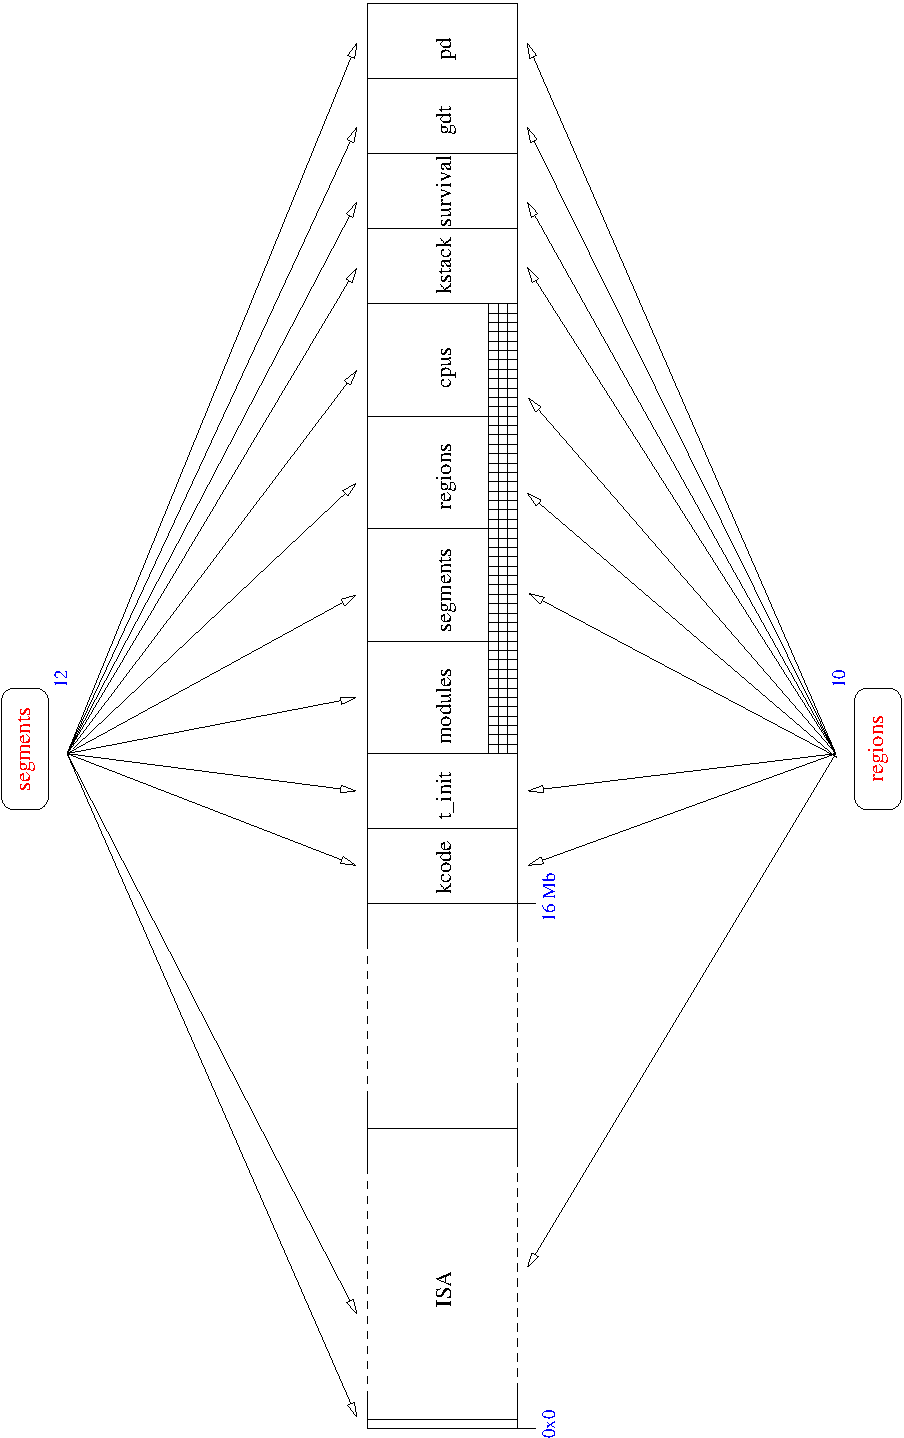
\includegraphics[angle=-90,width=\linewidth]{figures/k1-memory-layout.pdf}
\end{center}

The first segment (from 0 to 4 Kb) is used to prevent the mapping of
the first page when doing the identity mapping. This is used to detect
null-pointer dereferenciation.
